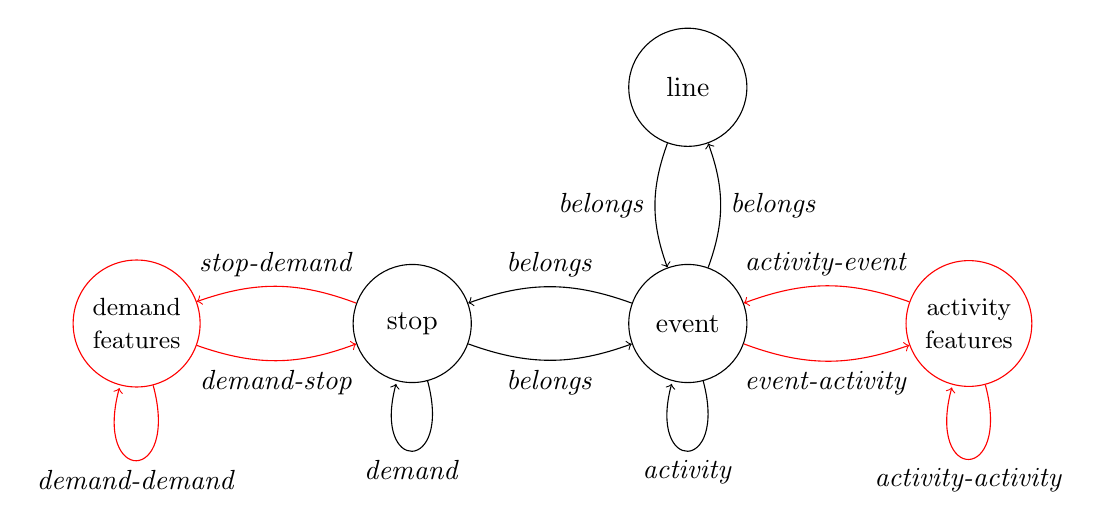
\begin{tikzpicture}[node distance=3.5cm, auto, swap]
    \tikzstyle{node}=[circle,draw, minimum size=1.5cm, align=center]
    \tikzstyle{node-red}=[circle,draw=red, minimum size=1.5cm, align=center]
    \node (event) [node] {event} edge [loop below] node {\textit{activity}} ();
    \node (stop) [node][left of=event] {stop} edge [loop below] node {\textit{demand}} ();
    \node (demand-type) [node-red] [left of=stop] {\small demand\\\small features} edge [loop below, draw=red] node {\textit{demand-demand}} ();;
    \node (activity-type) [node-red] [right of=event, xshift=2] {\small activity\\\small features} edge [loop below, draw=red] node {\textit{activity-activity}} ();
    \node (line) [node] [above of=event, node distance=3cm] {line};
    \draw [->, draw=red] (stop) to [bend right=20] node {\textit{stop-demand}} (demand-type);
    \draw [->, draw=red] (demand-type) to [bend right=20] node {\textit{demand-stop}} (stop);

    \draw [->, draw=red] (event) to [bend right=20] node {\textit{event-activity}} (activity-type);
    \draw [->, draw=red] (activity-type) to [bend right=20] node {\textit{activity-event}} (event);

    \draw [->] (stop) to [bend right=20] node {\textit{belongs}} (event);
    \draw [->] (event) to [bend right=20] node {\textit{belongs}} (stop);
    \draw [->] (event) to [bend right=20] node {\textit{belongs}} (line);
    \draw [->] (line) to [bend right=20] node {\textit{belongs}} (event);

    % \node {heimoi};
\end{tikzpicture}